\section{Résultats}
\label{sec:resultats}

\subsection{Première expérience}

Les résultats de la première expérience sont montrés dans la \figref{renaming}. Tout d'abord, le nombre de renommage varie beaucoup entre les projets. Par exemple, Jenkins a au plus $10\%$ de ses fichiers renommés dans la pire période alors que PHPUnit a deux périodes à plus de $50\%$. Le nombre de renommages varie aussi en fonction des périodes, par exemple dans PHPUnit la période $3.6 - 3.7$ a moins de $5\%$ de fichiers renommés alors que la période $3.7 - 4.0$ a presque $99\%$. En général, il y a beaucoup de périodes avec $0\%$ de fichiers renommés.\\

\begin{figure*}[h]
	\centering
	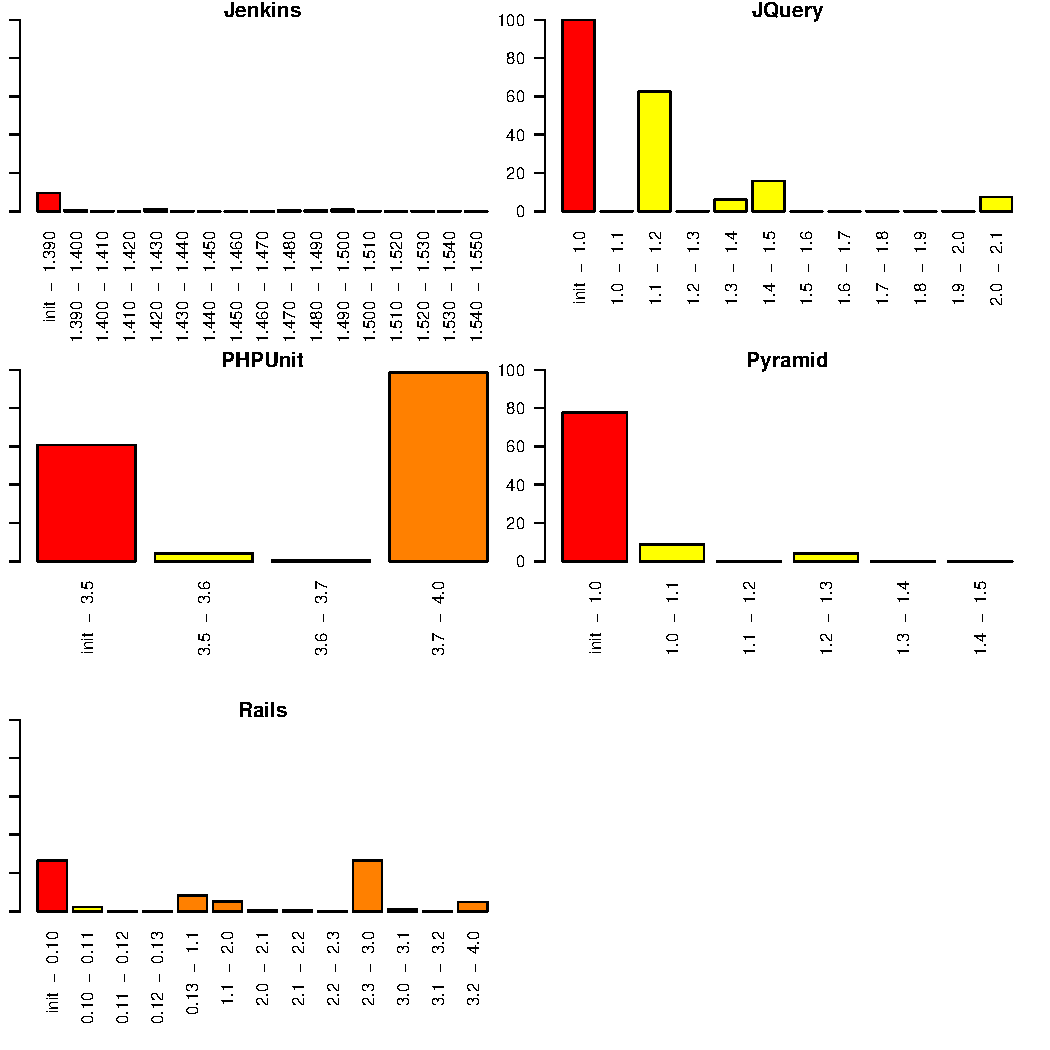
\includegraphics[width=0.85\linewidth,keepaspectratio]{data/figures/renaming.pdf}
	\caption{Pourcentage de fichiers renommés ($\%F_R$) dans chaque période de chaque projet de notre corpus. La période initiale est en gris foncé, les périodes majeures en gris et les périodes mineures en gris clair.}
	\label{fig:renaming}
\end{figure*}

Par rapport à la localisation de ces renommages, la période initiale semble la plus prolifique au renommage. En général, elle contient le plus grand nombre de fichiers renommés (sauf pour PHPUnit). Les périodes de développement sont plus susceptibles d'avoir des renommages que les périodes de maintenance. Ainsi, les $5$ projets sont quasiment à $0\%$ de fichiers renommés dans les périodes de maintenance. Finalement, certaines périodes de développement peuvent contenir beaucoup de renommages. Les résultats montrent que les releases majeures sont souvent les pires périodes de développement en nombre de fichiers renommés: C'est le cas pour PHPUnit et Rails alors que Jenkins et Pyramid ne contiennent pas de releases majeures.\\

%Le détail des résultats obtenus par notre outil de détection de renommage sont montrés dans les tables en annexes \tabref{jenkins}, \tabref{jquery}, \tabref{phpunit}, \tabref{pyramid} et %\tabref{rails}. Ces tables mettent en avant les valeurs suivantes:\\

%\begin{itemize}
%\item \emph{Nombre de fichiers ($\#F$):} nombre de fichiers dans le projet à la dernière version de la période..
%\item \emph{Nombre de fichiers actifs ($\#AF$):} nombre de fichiers créés, suprimés, copiés ou renommés durant la période et présents à la dernière version de la période.
%\item \emph{Pourcentage de fichiers actifs ($\%AF$):} $\%AF = \frac{\#AF}{\#F}$.
%\item \emph{Nombre de fichiers actifs renommés ($\#AF_{r}$):} nombre de fichiers actifs qui ont étés renommés.
%\item \emph{Pourcentage de fichiers renommés ($\%F_{R}$):} $\%F_{R} = \frac{\#AF_{R}}{\#F}$.
%\item \emph{Pourcentage de fichiers actifs renommés ($\%AF_{R}$):} $\%AF_{R} = \frac{\#AF_{R}}{\#AF}$.
%\end{itemize}

\subsection{Deuxième expérience}
Les résultats de notre deuxième expérience sont montrés dans la \tabref{spearman}. Ils montrent que la corrélation de coefficients de Spearman entre les métriques de procédés avec et sans détection de renommages dépendend beaucoup de la période et de la métrique choisie. Les métriques de procédés ne sont pas affectées par le renommage dans les projets Jenkins, Rails et Pyramid tels que le coefficient de corrélation est proche de $1$ dans tous les cas. D'un autre côté, pour PHPUnit et JQuery les métriques peuvent être sévèrement impactées par le renommage. Pour JQuery, la métrique Code Churn n'est pas affectée par le renommage, mais NoD et NoC sont quant à eux significativement impactés. Pour PHPUnit, toutes les métriques sont affectées par le renommage. Sur ces deux derniers projets, la métrique la plus sensible aux renommages de fichiers est le nombre de développeurs (NoD). Sur ces deux derniers projets, la métrique la plus sensible aux renommages de fichiers est le nombre de développeurs (NoD).

Finalement on peut noter que seules les périodes ayant eu un grand pourcentage de fichiers renommés ($\%F_R$) ont étés impactés. On peut aussi noter que des métriques biaisées par le renommage ont été calculées dans des releases majeures et mineures.\\

Nous avons étudié manuellement les deux périodes qui ont affecté les valeurs des métriques de procédés (JQuery 1.1 - 1.2 et PHPUnit 3.7 - 4.0). Par conséquent un grand nombre de fichiers ont étés renommés de manière transitive. C'est une pratique courante dans le développement logiciel, donc le phénomène pourrait apparaitre dans n'importe quelle période ou projet. Il est intéressent de noter que dans ces deux périodes les changements de structure ont été effectués en grande partie dans un seul commit proche de la fin de la période.\\


\begin{table*}[h]
\centering
\csvreader[tabular=rcccc, table head=\toprule & & \multicolumn{3}{c}{Change metrics}\\\cmidrule{3-5} Period & $\%F_R$ & CC & NoD & NoC\\\midrule, late after line=\\, late after last line=\\\bottomrule]{data/tables/correlations.csv}%
{1=\period,2=\fr,3=\churnall,4=\devall,5=\modificationsall}%
{\period & \fr & \churnall & \devall & \modificationsall}
\caption{La corrélation de coefficients de Spearman entre les valeurs des métriques de procédés avec et sans détection de renommage. Les codes de signification sont: *** $\leq 0.01$, ** $\leq 0.05$, * $\leq 0.1$ et ! $> 0.1$. Les coéfficiants moyen et faible sont affichés en gras.(TODO : gérer les tableaux)}
\label{tab:spearman}
\end{table*}


\subsection{Validations et limitations}


Our study makes the assumption that renamed files detected by Git tool are correct. However, we did not encounter any empirical evaluation of the Git renaming detection algorithm and therefore we have no confidence on its results. To mitigate this threat, we drew at random $100$ renamed files detected by Git in our corpus. We manually assessed each detected file renaming to check if it was correctly detected. Checking if a detected file renaming is correct consists in ensuring that the file content is very similar, and that no other file added in the same version has a similar content. This manual analysis revealed that $100\%$ of the detected renamed files were correctly detected. Even though we are aware that Git algorithm can yield false positives, this experiment shows that using Git as an oracle to detect renaming is reasonable. We did not analyzed the false negatives (true file renaming not detected by Git) as this is not a threat to our conclusion, since it will most likely lower the correlation coefficients if underestimated.\\

Due to a very small number of files, significance values of the correlation coefficients for the JQuery project are low for NoD and NoC. Nevertheless, significance of the correlation is not a threat with regard to our conclusion.\\

We only assessed the effect of renaming on three change metrics. The effect of renaming could be different (worse or better) for other change metrics. To mitigate this risk we used the most used change metrics as shown in~~\cite{radjenovic_software_2013}. Other change metrics are often based upon these metrics (such as \emph{code ownership}~\cite{bird_dont_2011} or \emph{module activity focus}~\cite{posnett_dual_2013}).\\

For the NoD metric, we did not apply an identity merging algorithm~\cite{goeminne_comparison_2013}. This could result in incorrect values. However, this phenomenon is likely to happen for both metrics with and without renaming, therefore the risk that it invalidates our conclusion is low.\\

Concerning our conclusion on the amount of renaming, the corpus we used do not guarantee that it is generalizable. Indeed, we only used open-source projects, while industrial projects are known to be significantly different. Regarding the validity among open-source projects, our corpus is to small to generalize our conclusion.
